%
% This is Chapter 2 file (chap2.tex)
%
\chapter{Kinetic theory and linear microkinetic instabilities}\label{chap:chap2}

    Kinetic theory forms a significant part of our understanding of plasma, specially at small
    scales (less than a $d_{\rm i}$). In this chapter, we give a brief overview of the salient
    properties of this theory. In \Cref{sec:intr2} we start with the equation of motion for a
    charged particle in an electromagnetic field and extend this idea to an ensemble of particles.
    In \Cref{sec:instab} we discuss anisotropy and linear instabilities arising because of it. We
    also discuss how one can compute rate of growth of these instabilities using kinetic theory. In
    \Cref{sec:app2} we discuss some of the application and observational evidence of linear theory.
    We finish this chapter with a brief discussion of limitations of linear theory in
    \Cref{sec:conc2}.

    \section{Introduction to Plasma Kinetic Theory} \label{sec:intr2}

        \subsection{Equations of motion}\label{sec:eqom}

            Consider a system which consists of a single charged particle of mass $m$ and charge $q$
            in a magnetic field $\mathbf{B}$ and an electric field $\mathbf{E}$. The
            non-relativistic equation of motion for this particle can then be written as:
            \begin{align}
                m \frac{d\mathbf{v}_1}{dt} & = q\left(\mathbf{E} + \mathbf{v}_1 \times \mathbf{B}\right) \label{eq:emot1}
            \end{align}
            and the its exact phase space\index{phase space} density at any point in space can be written as :
            \begin{align}
                \mathcal{F}_1(\mathbf{x},\mathbf{v},t) & = \delta \left(\mathbf{x}-\mathbf{x}_1(t)\right)\delta \left(\mathbf{v}-\mathbf{v}_1(t)\right) \label{eq:dens1}
            \end{align}
            where $\mathbf{x}_1(t)$ and $\mathbf{v}_1(t)$ are the position and velocity of the
            particle at any time $t$ and $\delta(...)$ is the Dirac delta function. The six
            dimensional space spanned by $\mathbf{x}$ and $\mathbf{v}$ is called phase
            space\footnote{Note: $\mathbf{x}$ and $\mathbf{v}$ are independent coordinates in phase
            space.}. If we have $n$ such particles in the system, then for the $i^\mathrm{th}$
            particle, \Cref{eq:emot1} can be written as :
            \begin{align}
                m_{\rm i} \frac{d\mathbf{v}_{\rm i}}{dt} & = q_{\rm i}\left(\mathbf{E}_\mu + \mathbf{v}_{\rm i} \times \mathbf{B}_\mu\right) \label{eq:emotn}
            \end{align}
            where the subscript $\mu$ represents the superposition of all the fields exerted by the
            particles in the system at the position of $i^\mathrm{th}$ particle. The total phase
            space density can now be written as:
            \begin{align}
                \mathcal{F}_{\rm n}(\mathbf{x},\mathbf{v},t) & = \sum_{i=1}^{n}\delta \left(\mathbf{x}-\mathbf{x}_{\rm i}(t)\right)\delta \left(\mathbf{v}-\mathbf{v}_{\rm i}(t)\right) \label{eq:densn}
            \end{align}
            In a closed system where there is no addition or removal of any particle, the total
            phase space density of a fluid element in phase space will remain constant in time.
            Using this conservation of phase space density one can write:
            \begin{align}
                \frac{d}{dt}\left(\mathcal{F}_{\rm n}(\mathbf{x},\mathbf{v},t)\right) & = 0 \label{eq:cons}
            \end{align}
            Since both $\mathbf{x}$ and $\mathbf{v}$ depend on time, we can use the chain rule and
            write \Cref{eq:cons} as:
            \begin{align}
            \frac{\partial \mathcal{F}_{\rm n}}{\partial t} + \frac{d \mathbf{x}}{d t} \cdot \frac{d \mathcal{F}_{\rm n}}{d \mathbf{x}} + \frac{d \mathbf{v}}{d t} \cdot \frac{d \mathcal{F}_{\rm n}}{d \mathbf{v}} & = 0 \label{eq:cons2}
            \end{align}
            where $\frac{\partial}{\partial t}$ is the partial derivative with respect to $t$. In
            \Cref{eq:cons2} we have dropped $(\mathbf{x},\mathbf{v},t)$ for the sake of readability.
            Using the fact that $\frac{d}{d t}\mathbf{x}=\mathbf{v}$ and substituting for $\frac{d
            \mathbf{v}}{d t}$ from \Cref{eq:emotn} in \Cref{eq:cons2}, we have:
            \begin{align}
            \frac{\partial \mathcal{F}}{\partial t} + \mathbf{v} \cdot \nabla_{\mathbf{x}} \mathcal{F} + \frac{q}{m}\left(\mathbf{E}_\mu + \mathbf{v} \times \mathbf{B}_\mu\right) \cdot \nabla_{\mathbf{v}} \mathcal{F} & = 0 \label{eq:cons3}
            \end{align}
            Solving \Cref{eq:cons3} (called the Klimontovich-Dupree equation) is quite a difficult
            task since it contains all the microscopic fields, the computation of which involves
            tracking the position and velocity of all the particles, which as we have already
            discussed is quite impossible to implement. This problem can be mitigated by writing the
            phase density as a sum of two parts, average and fluctuating as below:
            \begin{align}
                \begin{split}
                    \mathcal{F} & = \left<\mathcal{F}\right> + \delta\mathcal{F} \label{eq:pd1}\\
                    & = \mathnormal{f} + \delta\mathcal{F}
                \end{split}
            \end{align}
            where $\left<\mathcal{F}\right>$ denotes the smoothed average or the background value of
            $\mathcal{F}$, and $\delta \mathcal{F}$ is the fluctuation in the smoothed
            $\mathcal{F}$.  For ease of writing, from now on $\left<\mathcal{F}\right>$ will simply
            be denoted by $\mathnormal{f}$, which is also called the distribution function\index{distribution function} and is
            interpreted as the probability of finding a particle at any location within a phase
            space volume d\textbf{x}d\textbf{v}. If we carry out the same process for the fields, we
            can write them as:
            \begin{align}
                \begin{split}
                    \mathbf{E}_{\mu} & = \left<\mathbf{E}_{\mu}\right> + \delta\mathbf{E}_{\mu} \\
                    & = \mathbf{E} + \delta\mathbf{E}_{\mu}
                \end{split}
                \begin{split}
                    \mathbf{B}_{\mu} & = \left<\mathbf{B}_{\mu}\right> + \delta\mathbf{B}_{\mu} \\
                    & = \mathbf{B} + \delta\mathbf{B}_{\mu}\label{eq:pd2}
                \end{split}
            \end{align}
            Since $\mathcal{F}$, \textbf{B} and \textbf{E} are all smoothed averages, their
            fluctuations $(\delta\mathcal{F}, \delta\mathbf{B}, \delta\mathbf{E}$) will form an
            statistical ensemble which would imply that $\left<\delta ... \right> = 0$.

            Using \Cref{eq:pd1,eq:pd2} in \Cref{eq:cons3} and then taking the ensemble average, we
            have:
            \begin{align}
                \frac{\partial \mathnormal{f}}{\partial t} + \mathbf{v} \cdot \nabla_{\mathbf{x}}\mathnormal{f} + \frac{q}{m}\left(\mathbf{E} + \mathbf{v} \times \mathbf{B}\right) \cdot \nabla_{\mathbf{v}} \mathnormal{f} & = \frac{q}{m}\left<\left(\delta\mathbf{E} + \mathbf{v} \times \delta \mathbf{B}\right) \cdot \nabla_{\mathbf{v}} \mathcal{F}\right> \label{eq:kint}
            \end{align}
            This is the kinetic equation and defines the evolution of phase space density with time
            and position.

            Computing the right hand side of \Cref{eq:kint} is quite a difficult task, thus we often
            assume that the correlation between the background field and its fluctuation is
            infinitely small and collisions between particles account for correlation among
            themselves and occur uncorrelated of each other as random events, a consequence of the
            molecular chaos hypothesis\index{chaos hypothesis} (or
            \discolorlinks{\href{https://en.wikipedia.org/wiki/Boltzmann\_equation\#The\_collision\_term\_(Stosszahlansatz)\_and_molecular\_chaos}{\textit{sto\ss
            zahlansatz}}}) \citep{ClerkMaxwell1867}. Under these assumptions we can simply replace
            the right side of \Cref{eq:kint} with a collision operator\index{collision operator}, $\left(\frac{\partial
            \mathnormal{f}}{\partial t}\right)_{\rm c}$, which ideally will have all the information
            related to particle-particle interaction. \Cref{eq:kint} can thus be re-written as:
            \begin{align}
                \frac{\partial \mathnormal{f}}{\partial t} + \mathbf{v} \cdot \nabla_{\mathbf{x}}\mathnormal{f} + \frac{q}{m}\left(\mathbf{E} + \mathbf{v} \times \mathbf{B}\right) \cdot \nabla_{\mathbf{v}} \mathnormal{f} & = \left(\frac{\partial \mathnormal{f}}{\partial t}\right)_{\rm c} \label{eq:bolt}
            \end{align}
            This is the well known Boltzmann equation from statistical mechanics.
            \citet{Baumjohann1996} and references therein give some details about different
            functional forms of collisional operators\index{collision operator}.
            
            Presence of collision can significantly alter the shape of a VDF (see \Cref{sec:dfd} for
            definition). Since collisions can often result in transfer or exchange of energy and
            momentum between particles they work to erode the non-equilibrium features of a VDF
            (more on this later). In a fully ionized plasma where collisions are primarily coulombic
            in nature, computing the collision operator is further complicated by its dependence on
            temperature and density \citep{Baumjohann1996}. \citet{Landau1936} computed the
            collision operator, $\left(\frac{\partial \mathnormal{f}}{\partial t}\right)_{\rm c}$,
            for such a plasma, though solving it even for the simplest of cases is quite a daunting
            ask \citep{Verscharen2019}. However, \citet{Marsch1982, Marsch2010} showed that for
            space plasmas in the inner heliosphere collisions play negligible to minor role. We thus
            simply set the value of collision operator to zero and the Boltzmann equation
            (\Cref{eq:bolt}), in the absence of collision reduces to the Vlasov\index{Vlasov!equation} equation:
            \begin{align}
                \frac{\partial \mathnormal{f}}{\partial t} + \mathbf{v} \cdot \nabla_{\mathbf{x}}\mathnormal{f} + \frac{q}{m}\left(\mathbf{E} + \mathbf{v} \times \mathbf{B}\right) \cdot \nabla_{\mathbf{v}} \mathnormal{f} & = 0 \label{eq:vlas}
            \end{align}
            This equation forms the basis of much of kinetic theory for space plasmas and is used
            extensively in this thesis. We also use the Vlasov equation to derive the dispersion
            relation (see\,\Cref{sec:dpr}), which gives us an idea about the kind of waves and
            instabilities present in the system (more on this later).

        \subsection{Distribution Function and Other Definitions} \label{sec:dfd}

            As discussed in \Cref{sec:eqom}, $\mathnormal{f}(\mathbf{x,v},t)$ gives the probability
            density function (PDF)\index{distribution function!PDF} of particles in phase space. Different statistical moments of the
            PDF gives us macroscopic properties of the whole ensemble. Often, we are interested in
            the behaviour of the system at one particular position in the configuration space at any
            given time. This would mean that the PDF will have no dependence on the position
            (\textbf{x}) or any explicit dependence on time (t). We thus have a PDF with explicit
            dependence on just the velocity given as $\mathnormal{f}(\mathbf{v})$. This is referred
            to as velocity distribution function (VDF)\index{distribution function!VDF}. 

            For a VDF we can define some parameters associated with plasma using its statistical
            moments.\\
            \textbf{Density ($n_{\rm j}$)}: Number density of species $j$, usually expressed in the
            units of $\mathrm{cm^{-3}}$ and can be derived from VDF by computing its zeroth order
            moment as follows:
            \begin{align}
                n_{\rm j} = \int_{\forall \mathbf{v}} d^3\mathrm{v} \mathnormal{f}_{\rm j}\left(\mathbf{v}\right) \label{eq:numden}
            \end{align}
            \textbf{Bulk velocity\index{Bulk velocity} ($\mathbf{v}_{\rm j}$)}: The bulk velocity of the species $j$, or
            the mean particle velocity, usually has units of $\mathrm{km/sec}$ and can be derived
            from the VDF's first-order moment:
            \begin{align}
                \mathbf{v}_{\rm j} = \frac{1}{n_{\rm j}}\int_{\forall \mathbf{v}} d^3\mathrm{v} \mathbf{v} \mathnormal{f}_{\rm j}\left(\mathbf{v}\right) \label{eq:blkvel}
            \end{align}
            \textbf{Thermal Speed\index{Thermal Speed} ($w_{\rm j}$)}: It represents the thermal speed of the species j
            and has units of $\mathrm{km/sec}$. It is a measure of thermal energy of species $j$ and
            the value for it can be derived from the VDF's second-order moment:
            \begin{align}
                \mathrm{v}_{\rm j}^2 + 3\,w_{\rm j}^2 = \frac{1}{n_{\rm j}}\int_{\forall \mathbf{v}} d^3\mathrm{v} \mathbf{v}^2 \mathnormal{f}_{\rm j}\left(\mathbf{v}\right) \label{eq:wtherm}
            \end{align}
            For an anisotropic case, where temperature is different along different directions,
            \Cref{eq:wtherm} is computed for each component separately (see \citet[\S
            1.4.1]{Verscharen2019} for a detailed description).\\
            \\
            \textbf{Temperature ($T_{\rm j}$)}: Using the thermal speed, one can define the
            temperature (in units of K) of the species as:
            \begin{align}
                T_{\rm j} & = \frac{m_{\rm j}\,w_{\rm j}^2}{2k_{\rm B}} \label{eq:temp}
            \end{align}
            In a magnetized plasma, the VDFs commonly exhibit distinct temperatures perpendicular
            and parallel to the magnetic field because of the slightly different heating or cooling
            rates in different directions \citep{Stix1992, Gary1993}. We thus have different
            temperatures in parallel ($T_{\rm \parallel j}$) and perpendicular ($T_{\rm \perp j}$)
            directions and the total temperature of species j is then given as:
            \begin{align}
                 T_{\rm j} = \frac{T_{\rm \parallel j} + 2 T_{\rm \perp j}}{3} \label{eq:ttemp}
            \end{align}
            The ratio of two temperatures (perpendicular and parallel) is called anisotropy\index{anisotropy} and is
            expressed as:
            \begin{align}
                 R_{\rm j} = \frac{T_{\rm \rm \perp j}}{T_{\rm \parallel j}} \label{eq:aniso}
            \end{align}
            \textbf{Parallel Beta ($\beta_{\rm \parallel j}$)}: It is the ratio of parallel thermal
            energy of a species to the magnetic pressure energy stored in the field.
            \begin{align}
                \beta_{\rm \parallel j} = \frac{n_{\rm j}\,k_{\rm B}\,T_{\rm \parallel j}}{B_0^2/(2\mu_\circ)} \label{eq:beta}
            \end{align}
            As we will see later in this chapter (see \Cref{sec:instab2}) the values of parameters
            $R_{\rm j}$ and $\beta_{\rm \parallel j}$ play an important role in determining if a
            region of plasma is stable or unstable. \\
            \\
            \textbf{Shape of a VDF}:\\
            In general the VDF can take a variety of forms as long as they conform to the laws of
            probability. For a plasma in local thermodynamic equilibrium, it takes the shape of a
            Maxwellian distribution\index{distribution function!Maxwellian} as shown in \Cref{eq:vdf}.
            \begin{align}
                \mathnormal{f}_{\rm j}(\mathbf{v}) & = \frac{n_{\rm j}}{\left(\pi w_{\rm j}^2\right)^{3/2}} \mathrm{exp}\left(-\frac{\left|\mathbf{v} - \mathbf{v}_{\rm 0}\right|^2}{w_{\rm j}^2}\right) \label{eq:vdf}
            \end{align}
            where $\mathbf{v}_{\rm 0}$ is the streaming velocity of the plasma. Each species ($j$)
            in the plasma has its own VDF, the statistical moments of which give the species' bulk
            parameters (e.g., density and velocity).

            One can define a direction based on the background field present in the plasma. If we
            assign the direction along the magnetic field as the parallel direction (represented by
            $\parallel$) and the other two orthogonal directions as the perpendicular direction
            (represented by $\perp$), the total magnetic field can be expressed in this new
            coordinate system as:
            \begin{align}
                \mathbf{B} = B_\parallel\,\mathbf{\hat{e}}_\parallel + B_\perp\,\mathbf{\hat{e}}_\perp \label{eq:newdir}
            \end{align}
            where $\mathbf{\hat{e}}_\parallel~\mathrm{and}~\mathbf{\hat{e}}_\perp$ are the unit
            vectors along and perpendicular to the magnetic field.

            It is often easier to work with VDFs in this coordinate system, thus we rewrite
            \Cref{eq:vdf} for a species $j$ in the new coordinate system as:
            \begin{align}
                \mathnormal{f}_{\rm j}(\mathbf{v}) & = \frac{n}{\pi^{3/2} w_{\rm \perp j}^2 w_{\rm \parallel j}} \mathrm{exp}\left(-\frac{(\mathrm{v}_\parallel - \mathrm{v}_{\rm \parallel 0j})^2}{w_{\rm \parallel j}^2} -\frac{|\mathbf{v}_\perp - \mathbf{v}_{\rm \perp 0j}|^2}{w_{\rm \perp j}^2}\right) \label{eq:vdf2}
            \end{align}
            The values of $\mathbf{v}_{\rm \parallel 0j}$ and $\mathbf{v}_{\rm \perp 0j}$ are often
            different resulting in a slightly different VDF in the two directions. For such a case,
            the VDF is referred to as the bi-Maxwellian\index{distribution function!bi-Maxwellian} distribution.
            
            Though in this thesis we use \Cref{eq:vdf2} as the standard/default VDF unless otherwise
            stated, it must be noted that for solar wind, especially at 1\,au, the VDF departs
            significantly from a simple bi-Maxwellian \citep{Feldman1974, Feldman1974a, Marsch1982b,
            Alterman2018}. Ion VDFs often have an asymmetry which can be more accurately accounted
            for by superposition of a differentially flowing bi-Maxwellian \citep{Alterman2018}.
            Other forms of distribution such as kappa distribution has also been used to study the
            non-Maxwellian features of VDF like enhanced tail \citep{Pierrard2010,Pierrard2014,
            Maksimovic1997,Nicolaou2020}.

    \section{Linear Microkinetic Instabilities} \label{sec:instab}

        \subsection{The Linear Dispersion Relation} \label{sec:dpr}
 
            Though in \Cref{sec:eqom} we made several assumptions and used our a priori knowledge of
            the system, solving \Cref{eq:vlas} for even a simple distribution like the bi-Maxwellian
            (\Cref{eq:vdf2}) is quite complicated and computationally expensive. Coupling between
            fields produced by one species with another species complicates it further.
            Linearization (or linear analysis), where one assumes plain wave perturbation in fields
            and the VDF helps simplify the problem while keeping the underlying physics of the
            equations intact as long as the fluctuations have small amplitude relative to the
            background values. In standard linear theory, we assume an equilibrium (i.e., constant)
            background and perturb it with a small-amplitude sinusoidal fluctuation of wave vector
            \textbf{k} and angular frequency $\omega$. The goal then is to derive, for a given
            plasma, the dispersion relation: the relationship between \textbf{k} and $\omega$. Under
            this assumption one can rewrite \Cref{eq:pd1,eq:pd2} as:
            \begin{align}
                \begin{split}
                    \mathnormal{f}_{\rm j}(\mathbf{x}, \mathbf{v}, t) & = \mathnormal{f}_{\rm j}^0(\mathbf{x}, \mathbf{v}) + \mathnormal{f}_{\rm j}^1(\mathbf{x}, \mathbf{v}, t)\\
                    & = \mathnormal{f}_{\rm j}^0(\mathbf{x}, \mathbf{v}) + \mathnormal{f}_{\rm j}^1(\mathbf{k}, \omega, \mathbf{v})~e^{(i(\mathbf{k}\cdot \mathbf{x} -\omega t))}\label{eq:vdfn1}
                \end{split}
            \end{align}
            \vspace{-0.4cm}
            \begin{align}
                \begin{split}
                    \mathbf{B}(\mathbf{x}, t) & = \mathbf{B}^0(\mathbf{x}) + \mathbf{B}^1(\mathbf{x}, t)\\
                    & = \mathbf{B}^0(\mathbf{x}) + \mathbf{B}^1(\mathbf{k},\omega)~e^{(i(\mathbf{k}\cdot \mathbf{x} -\omega t))}\label{eq:mag1}
                \end{split}
            \end{align}
            \vspace{-0.4cm}
            \begin{align}
                \begin{split}
                    \mathbf{E}(\mathbf{x}, t) & = \mathbf{E}^0(\mathbf{x}) + \mathbf{E}^1(\mathbf{x}, t)\\
                    & = \mathbf{E}^0(\mathbf{x}) + \mathbf{E}^1(\mathbf{k},\omega)~e^{(i(\mathbf{k}\cdot \mathbf{x} -\omega t))}\label{eq:efl1}
                \end{split}
            \end{align}
            Where $\mathbf{k}$ and $\omega$ are the wavenumber vector and the frequency of
            perturbation, respectively. \Crefrange{eq:vdfn1}{eq:efl1} along with Maxwell's
            equation's (\Crefrange{eq:maxwell1}{eq:maxwell4}) help us drive the dispersion
            relations. In order to do so, we start with some simple assumptions and conditions. We
            work in a frame of reference where the zeroth order current density
            ($\mathbf{J}^0(\mathbf{x})$) and electric field ($\mathbf{E}^0(\mathbf{x})$) are zero
            and the magnetic field ($\mathbf{B}^0(\mathbf{x})$) is constant. Thus
            \Cref{eq:mag1,eq:efl1} can be rewritten as:
            \begin{align}
                \mathbf{B}(\mathbf{x}, t) & = \mathbf{B}_{\rm 0} + \mathbf{B}^1(\mathbf{x}, t)\label{eq:mag2}\\
                \mathbf{E}(\mathbf{x}, t) & = \mathbf{E}^1(\mathbf{x}, t)\label{eq:efl2}\\
                \mathbf{J}(\mathbf{x}, t) & = \mathbf{J}^1(\mathbf{x}, t)\label{eq:curr2}
            \end{align}
            We choose a co\"ordinate system with $z$-axis along the background magnetic field
            ($\mathbf{B}_{\rm 0}$). The angle between the direction of propagation of fluctuation
            ($\mathbf{k}$) and the magnetic field is:
            \begin{align}
                \cos \left(\theta \right) & = \frac{\mathbf{k}\cdot\mathbf{B}}{k B}\label{eq:theta}
            \end{align}
            Substituting expressions for $\mathbf{J}, \mathbf{B}~\mathrm{and}~\mathbf{E}$ into
            Maxwell's equations (\Crefrange{eq:maxwell1}{eq:maxwell4}) and simplifying we have:
            %by substituting $\frac{\partial}{\partial t}$ with $\omega$ and $\nabla$ with
            %$\mathbf{k}$, we get:
            \begin{align}
                \mu_\circ\,\mathbf{J}^1(\mathbf{k}, \omega) & = \frac{i}{\omega}\,\mathbf{k} \times \left[\mathbf{k} \times \mathbf{E}^1(\mathbf{k}, \omega)\right] + \frac{i\,\omega}{c^2}\,\mathbf{E}^1(\mathbf{k}, \omega) \label{eq:curr3}
            \end{align}
            In similar fashion to the particle velocity in \Cref{eq:blkvel} one can write the flux
            density as:
            \begin{align}
                \Gamma_{\rm j}^1(\mathbf{k}, \omega) = \int_{-\infty}^{\infty}d^3 v\,\mathbf{v}\,\mathnormal{f}_{\rm j}^1(\mathbf{k}, \omega, \mathbf{v}) \label{eq:flux1}
            \end{align}
            and thus define the current density as:
            \begin{align}
                \mathbf{J}^1(\mathbf{k}, \omega) & = \sum_{\rm j} q_{\rm j}\,\mathbf{\Gamma}_{\rm j}^1(\mathbf{k}, \omega) \label{eq:curr4}
            \end{align}
            For species $j$ we can define the dimensionless conductivity tensor $\mathbf{S}_{\rm j}$
            as:
            \begin{align}
                \mathbf{\Gamma}_{\rm j}^1(\mathbf{k}, \omega) & = - \frac{i\,\epsilon_\circ\,k^2\,c^2}{q_{\rm j}\,\omega}\,\mathbf{S}_{\rm j}(\mathbf{k},\omega)\cdot \mathbf{E}^1(\mathbf{k},\omega) \label{eq:curr5}
            \end{align}
            Combining \Cref{eq:curr2,eq:curr3,eq:curr4} gives us:
            \begin{align}
                \mathbf{D}(\mathbf{k},\omega)\cdot \mathbf{E}^1(\mathbf{k},\omega) & = 0 \label{eq:disp1}
            \end{align}
            where,
            \begin{align}
                \mathbf{D}(\mathbf{k},\omega) = \left(\omega^2 - c^2\,k^2\right)\mathbf{I} + c^2\,\mathbf{k}\,\mathbf{k} + c^2\,k^2\,\sum_{\rm j}\,\mathbf{S}_{\rm j}(\mathbf{k},\omega) \label{eq:disp2}
            \end{align}
            with \textbf{I} being the 3-dimensional identity matrix and \textbf{k}\,\textbf{k} being
            the dyadic\footnote{The dyadic product between two vectors \textbf{a} and \textbf{b} is
            simply the product between the vector and its transpose, so one has
            $\mathbf{a}\,\mathbf{b} = \mathbf{a}\,\mathbf{b}^T$, which results in a rank-two
            tensor.} product of the wavevector. For \Cref{eq:disp2} to be true, $\mathbf{E}^1$
            cannot be allowed to go to zero since that would allow perturbations in the system to
            vanish. Hence we must have the determinant of $\mathbf{D}(\mathbf{k},\omega)$ go to
            zero, thus:
            \begin{align}
                \mathrm{det}(\mathbf{D}(\mathbf{k},\omega)) & = 0 \label{eq:disp3}
            \end{align}
            which is the plasma dispersion relation\index{dispersion relation}. \citet{Gary1993} notes that this equation can
            be solved ``either as a boundary value problem ($\omega$ is given as real, one solves
            for a complex component of $\mathbf{k}$) or as an initial value problem ($\mathbf{k}$ is
            given as real, one solves for complex $\omega$)''.
            
            \Cref{eq:disp3} in general gives infinite number of solutions for $\omega$ for any value
            of \textbf{k} and a set of plasma parameters. Thus $\omega (\mathbf{k})$ is a multi
            valued function with multiple branches corresponding to different modes (see
            \citet[Figure 2]{Schwartz1980}). However most modes are strongly damped and thus
            dissipate before they can substantially effect the plasma.

        \subsection{Temperature Anisotropy Induced Instabilities} \label{sec:instab2}

            In a homogeneous plasma (PDF is independent of position) in local thermodynamic
            equilibrium (LTE), all fluctuations (at any \textbf{k} and $\omega$) are damped and thus
            have a decaying amplitude. However, departure from LTE because of the non-Maxwellian
            properties of VDFs (temperature anisotropy or relative drift between two different
            species, etc.) introduce free energy into the system. This results in circumstances
            where instead of getting damped some perturbations grow exponentially and make the
            system unstable. The rate at which such a perturbation propagates and gets damped or
            grows is computed by solving the dispersion relation (\Cref{eq:disp3}). Solutions of
            \Cref{eq:disp3} using the initial value problem method gives $\omega$, which is in
            general complex and can be written as:
            \begin{align}
                \omega = \omega_{\rm r} + i \gamma \label{eq:omega}
            \end{align}
            where, $\omega_{\rm r}$ is the real component and $\gamma$ is the damping rate ($\gamma
            < 0$) or growth rate\index{microinstability!growth rate} ($\gamma > 0$). In the presence of a growth rate, the fluctuations
            present in the system start to grow exponentially. If the process continues,
            fluctuations start having amplitudes comparable to the background value, which makes the
            assumption of linearity void and makes the system non-linear. The state of the system
            can no longer be predicted by linear theory and instead relies on non-linear dynamics.

            When an instability has $\gamma = 0$ for any wave vector, we call it threshold\index{threshold} of the
            associated instability. We also define $\gamma_{\max}$ for a given branch of dispersion
            solutions as the maximum value of $\gamma$ for different wavenumbers ($\mathbf{k}$) and
            for all propagation directions ($\theta$). $\omega_{max}$ and $\mathbf{k}_{\max}$ are
            then defined as the values of $\omega$ and $\mathbf{k}$ corresponding to $\gamma =
            \gamma_{\max}$ respectively. Mathematically this can be written as:
            \begin{align}
                \begin{split}
                    \gamma_{\max}^j = \mathrm{\max}\left(\gamma^j\left(\mathbf{k},\theta\right)\right)~~\forall \left(\mathbf{k}, \theta\right) \label{eq:gammamax}
                \end{split}
            \end{align}
            where $j$ represents the branch of dispersion solutions for which $\gamma$ was computed.

            In this thesis we consider ion temperature anisotropy as the only source of free energy.
            For instability driven by ion temperature anisotropy, there are four distinct modes
            depending on the anisotropy value ($R_{\rm p}$) and the direction of propagation
            ($\theta$). For parallel propagation ($\theta=0$), there are two modes: ion cyclotron
            for $R_{\rm p} > 1$ and parallel firehose for $R_{\rm p} < 1$. In the oblique direction
            ($0 < \theta < 90$), the corresponding instabilities are mirror ($R_{\rm p} > 1$) and
            oblique firehose ($R_{\rm p} < 1$). It is worth noting that neither of these two oblique
            instabilities propagate. \Cref{tab:instab} gives a summary of all four instabilities
            discussed.

            \begin{table}[ht]
                \centering
                \caption[Microkinetic instabilities]{List of four temperature-anisotropy induced instabilities in plasma}
                \begin{tabular}{ | p{0.25\linewidth} | p{0.25\linewidth} | p{0.25\linewidth}| }
                    \hline
                    Anisotropy Range & Parallel ($\omega_{\rm r} > 0$) & Oblique ($\omega_{\rm r} =
                    0$)\\
                    \hline
                    $R_{\rm p} > 1$ & Ion cyclotron & Mirror\\
                    \hline
                    $R_{\rm p} < 1$ & Parallel firehose & Oblique firehose\\
                    \hline
                \end{tabular}
                \label{tab:instab}
            \end{table}

        \subsection{Computing Growth Rates}\label{sec:cgr}

            Computation of growth rates ($\gamma$) for any given value of the plasma parameters for
            a given branch of instability means solving \Cref{eq:disp3} for all different values of
            \textbf{k}. This is generally done by using a numerical dispersion solver. This project
            used tables of $\gamma_{\max}$ as a function of the plasma parameters developed by
            \citet{Maruca2012} using the software of \citet{Gary1993}. For our case, given a value
            of $R_{\rm p}$ and $\beta_{\parallel \rm p}$, we check the table for values of ($R_{\rm
            p}, \beta_{\parallel \rm p}$) that are closest to the input value and then use an
            interpolation technique (cubic spline interpolation) to get the value at that exact
            input point.

            Once we get the $\gamma_{\max}$ value corresponding to an instability, we normalize it
            to the cyclotron frequency of protons ($\gamma_{\max} \rightarrow
            \gamma_{\max}/\Omega_{\rm cp}$). However, not all computed values of the growth rate
            will have a significant effect on the plasma dynamics. As is expected if growth rate is
            high, the instability grows faster and conversely it will take the instability a long
            time to manifest or change the dynamics if it has a small growth rate. Thus, one can
            think of $1/\gamma$ as a proxy for the amount of time it will take for the instability
            to manifest itself. For a positive but an infinitesimal value of $\gamma_{\max}$, the
            value of time will be much, much greater than the other characteristic time scales of
            the system, which means the instability will never have time to significantly affect the
            plasma. We thus define a cut-off\index{microinstability!cut-off} value of growth rates, in units of proton cyclotron
            frequency, as:
            \begin{align}
                \gamma_{\max, \mathrm{cut\textrm{-}off}}^j & = 10^{-5}\,\Omega_\mathrm{{cp}} \label{eq:gammacutoff}
            \end{align}
            For any combination of ($R_{\rm p}, \beta_{\parallel \rm p}$) if the value of
            $\gamma_{\max}/\Omega_\mathrm{{cp}}$ is less than $10^{-5}$ we essentially set those
            values to zero and assume that the plasma is completely stable at those points. Choosing
            this cut-off is a bit arbitrary. Different studies have chosen different threshold
            values. For example \citet{Gary1999} and \citet{Gary2006} chose $\gamma =
            10^{-2}\,\Omega_{\rm cp}$ as their cut-off, whereas both \citet{Hellinger2006} and
            \citet{Klein2018} settled on cut-off value of $\gamma = 10^{-3}\,\Omega_{\rm cp}$. As
            long as the cut-off value of $\gamma$ is significantly smaller than that of other
            relevant time scales (see \Cref{sec:nlts,sec:data7}) it can comfortably be set to zero.

    \section{Application of linear theory and observational evidence}\label{sec:app2}

        The low density and extreme dynamics of space plasmas, such as  solar wind and the
        magnetosheath (see \Cref{sec:plas2}), ensure that they almost invariably deviate
        substantially from local thermal equilibrium \citep{Marsch2006a,Verscharen2019}. For
        example, even though the majority of solar wind ions are protons (ionized hydrogen) or
        $\alpha$-particles (fully ionized helium), these two particle species rarely have equal
        temperatures or bulk velocities \citep[see,
        e.g.,][]{Feldman1974a,Marsch1982,Hefti1998,Kasper2008,Maruca2013a}. \Cref{fig:temp_1au}
        shows the distribution of temperature for these two species using data from the Wind
        spacecraft (\Cref{sec:wind} for more details on the dataset used). Furthermore, the VDF of
        any given ion species often significantly departs from the entropically favored Maxwellian
        functional form \citep{Feldman1973a,Feldman1974,Marsch1982b, Alterman2018}. Observations of
        solar wind and magnetosheath from multiple spacecraft
        \citep{Feldman1973b,Marsch1982b,Kasper2002} have shown that the protons exhibit distinct
        kinetic temperatures, $T_{\rm \perp p}$ and $T_{\rm \parallel p}$. Both values of $R_{\rm p}
        > 1$ and $R_{\rm p} < 1$ are commonly observed in the solar wind and in Earth's
        magnetosheath, making it an ideal candidate for the application of linear Vlasov theory\index{Vlasov!linear Vlasov theory}.
        \Cref{fig:aniso_wnd_mms} shows distribution of $R_{\rm p}$ for solar wind at 1\,au and
        magnetosheath.
        \begin{figure}
            \begin{center}
                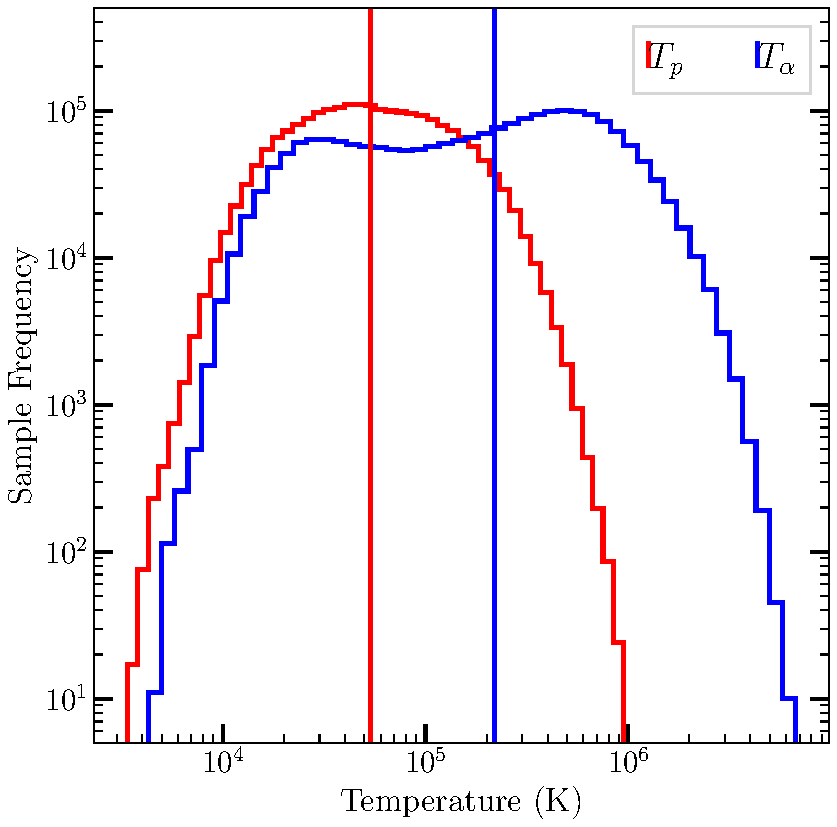
\includegraphics[width=0.55\textwidth]{figures/chap2/proton_alpha_temp_dist_wnd.pdf}
                \caption[Temperature distribution at 1\,au]{Distribution of proton and $\alpha$-temperatures at 1\,au. Vertical lines show the median temperature of each species.}
                \label{fig:temp_1au}
            \end{center}
        \end{figure}

        \begin{figure}
            \begin{center}
                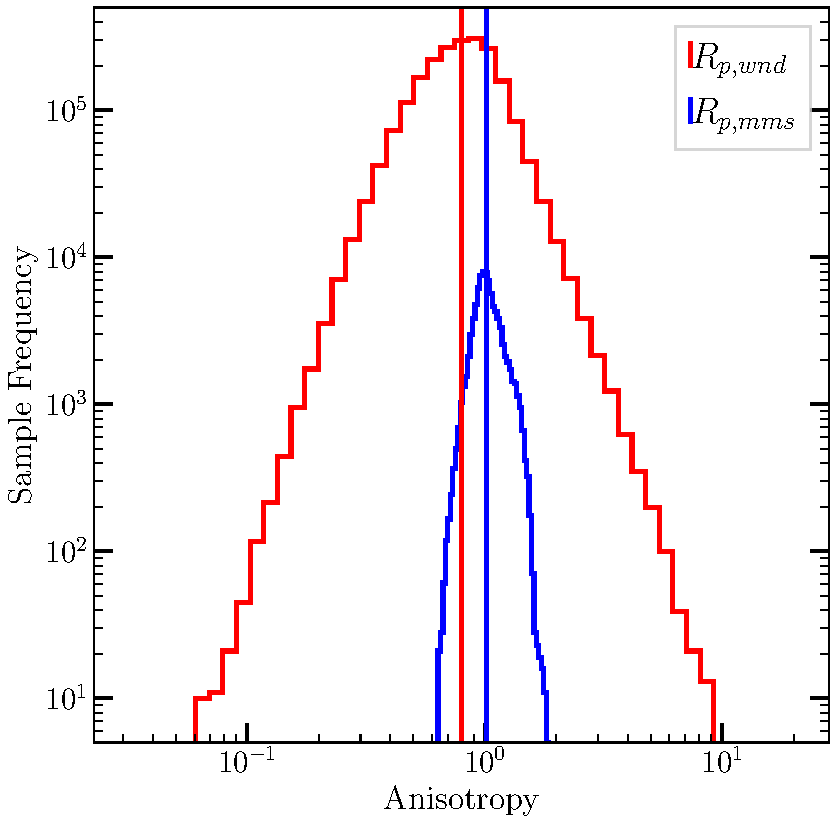
\includegraphics[width=0.55\textwidth]{figures/chap2/proton_aniso_dis_mms_wnd.pdf}
                \caption[$R_{\rm p}$ distribution at 1\,au and in magnetosheath]{Distribution of proton temperature anisotropy at 1\,au (red) and in the magnetosheath (blue). Vertical lines show the median values at each location.}
                \label{fig:aniso_wnd_mms}
            \end{center}
        \end{figure}

        As discussed in \Cref{sec:instab2} if $R_{\rm p}$ departs sufficiently from unity, it can
        trigger a kinetic microinstability\index{microinstability}: a short-wavelength fluctuation with an exponentially
        growing amplitude. The threshold $R_{\rm p}$-value for the onset of a proton
        temperature-anisotropy instability depends on all plasma parameters (e.g., composition and
        relative temperatures), depending most strongly on proton parallel beta ($\beta_{\parallel
        \rm p}$). \Cref{fig:gamma_cntr} shows various thresholds on an ($R_{\rm p}, \beta_{\rm
        \parallel p}$) plane for the four modes of instabilities. As is evident, at fixed $R_{\rm
        p}$ a slight increment in $\beta_{\parallel \rm p}$ can lead to significant increase in the
        growth rate.

        \begin{figure}
            \begin{center}
                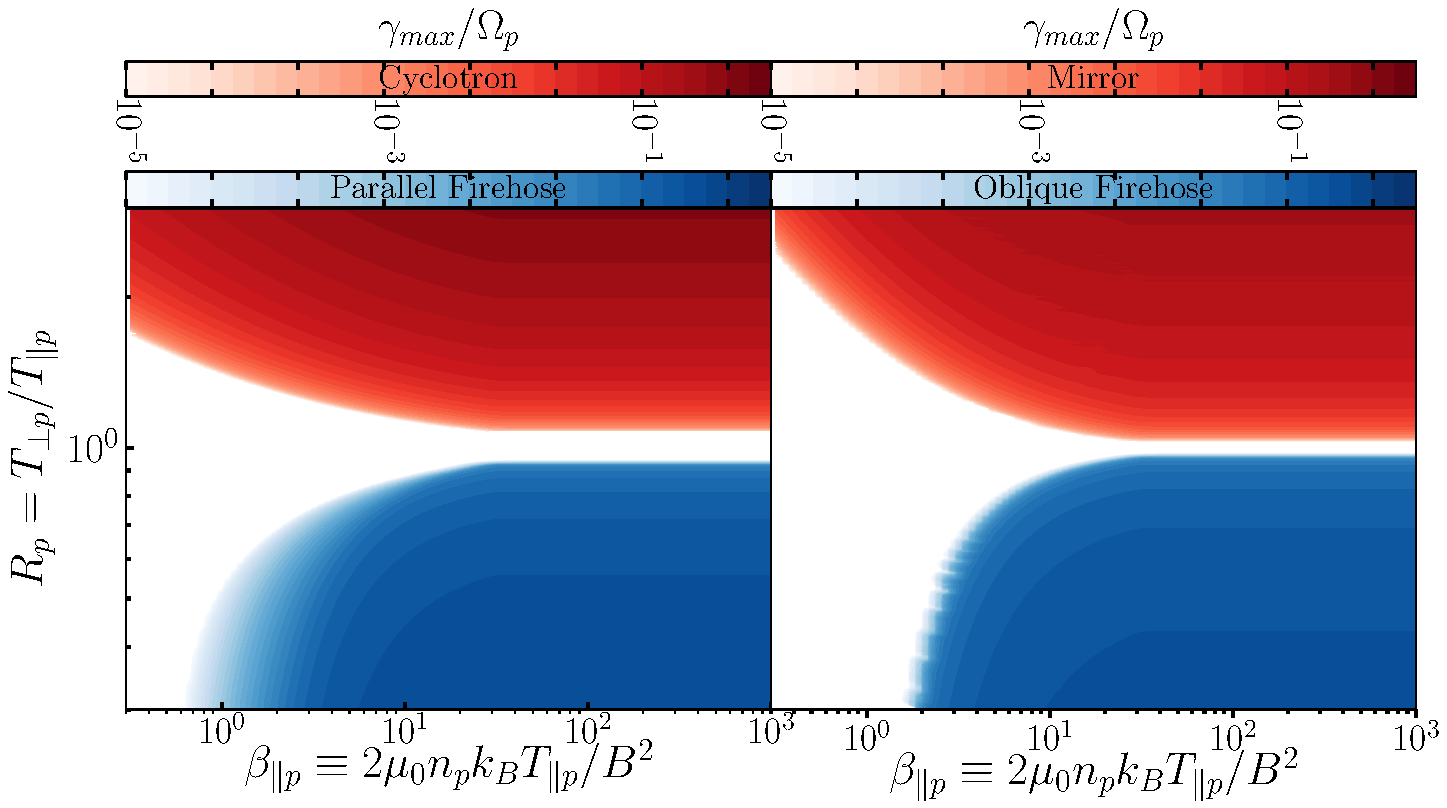
\includegraphics[width=1\textwidth]{figures/chap2/growth_rate_contours.pdf}
                \caption[$\gamma$ Contours]{Contours of constant growth rates.}
                \label{fig:gamma_cntr}
            \end{center}
        \end{figure}

        These instabilities have threshold $R_{\rm p}$-values, which means that they can effectively
        limit the degree to which proton temperature can depart from isotropy. If an unstable mode
        grows and does not saturate, it eventually becomes nonlinear, continues to scatter particles
        in phase space, and eventually drives the VDF toward local thermal equilibrium. Multiple
        studies have analyzed large datasets from various spacecraft and under the assumptions of a
        spatially homogeneous plasma and a bi-Maxwellian proton velocity distribution; such studies
        have found that the joint distribution of $(\beta_{\parallel \rm p},R_{\rm p})$-values from
        the interplanetary solar wind largely conform to the limits set by the instability
        thresholds \citep{Gary2001,Kasper2002,Hellinger2006,Matteini2007}.
        \Cref{fig:brazil_prob_wnd} shows the joint probability distribution of ($R_{\rm p},
        \beta_{\parallel \rm p}$) and the thresholds\index{threshold} corresponding to different instability modes
        for $\gamma_{\max}/\Omega_{\rm cp} = 10^{-2}$ \footnote{Please see \Cref{apdx:A} for more
        details on how these figures were made and how thresholds were computed}. We can see that
        the probability density decreases significantly as one moves closer to any of the threshold
        values. A recent study by \citet{Maruca2018} confirmed the same effect in Earth's
        magnetosheath, which is shown in \Cref{fig:brazil_prob_mms} (see \Cref{apdx:A} for examples
        of a $(\beta_{\parallel \rm p},R_{\rm p})$-plot in other systems). Additional studies have
        found that plasma with unstable $(\beta_{\parallel \rm p},R_{\rm p})$-values is
        statistically more likely to exhibit enhancements in magnetic fluctuations \citep{Bale2009}
        and proton temperature \citep{Maruca2011}. These findings suggest that the instabilities not
        only regulate temperature anisotropy in space plasmas but, in doing so, play an integral
        role in the large-scale evolution of the plasmas.

        \begin{figure}
            \begin{center}
                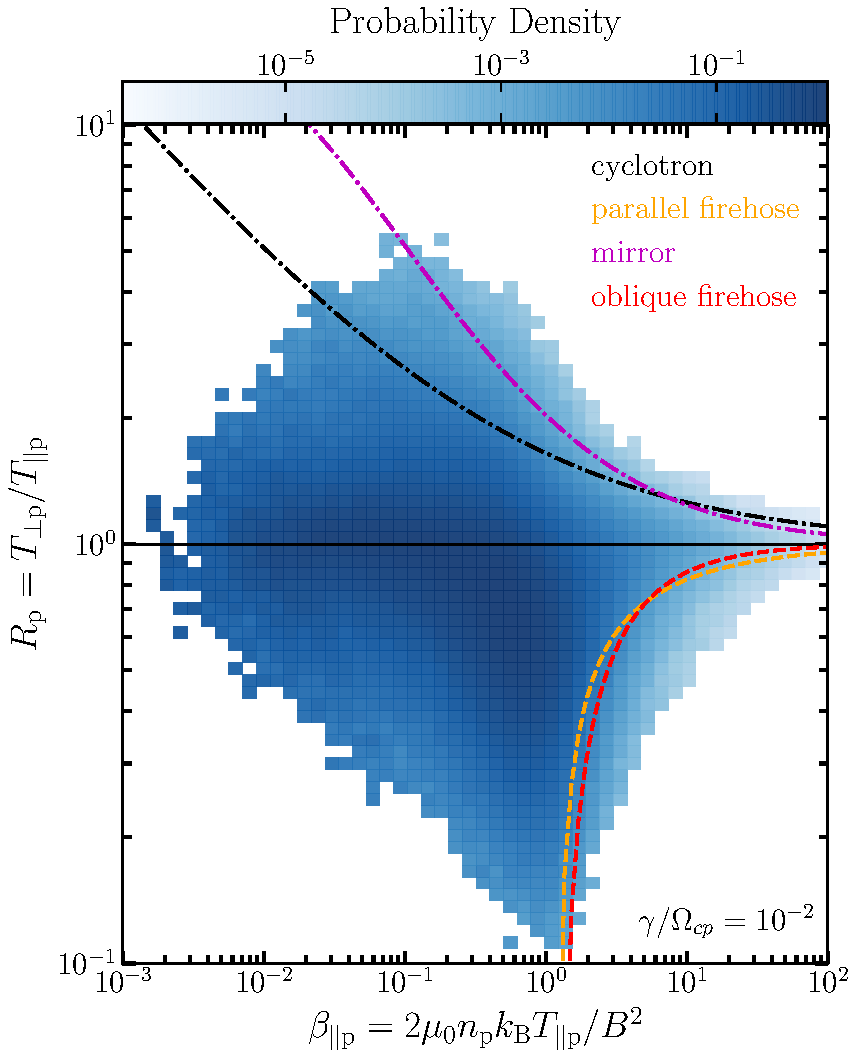
\includegraphics[width=1\textwidth]{figures/chap2/brazil_prob_wnd.pdf}
                \caption[Brazil-plot at 1\,au]{Plot of estimated probability density, $\Tilde{p}$ of
                ($R_{\rm p}, \beta_{\parallel \rm p}$) for solar wind at 1\,au (from \texttt{wnd}
                dataset, see \Cref{chap:chap4}) and thresholds associated with different
                instabilities for threshold value of $\gamma_{\max}/\Omega_{\rm cp} = 10^{-2}$.}
                \label{fig:brazil_prob_wnd}
            \end{center}
        \end{figure}
        \begin{figure}
            \begin{center}
                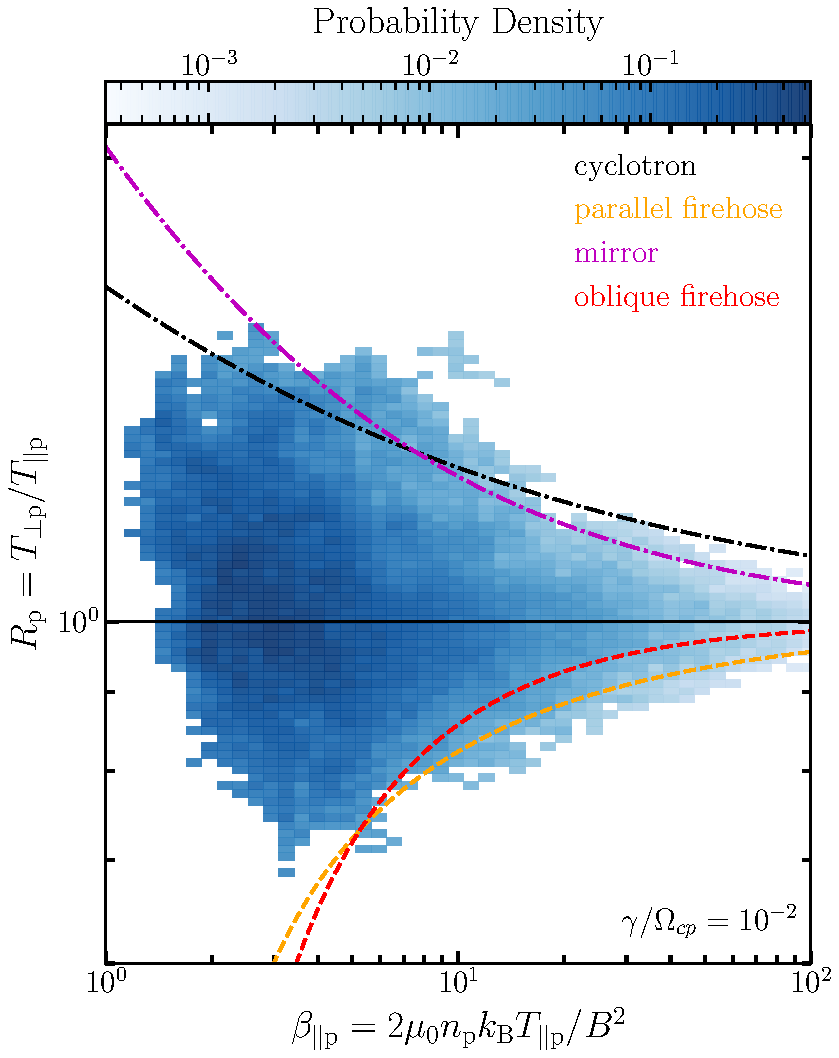
\includegraphics[width=1\textwidth]{figures/chap2/brazil_prob_mms.pdf}
                \caption[Brazil-plot in magnetosheath]{Plot of estimated probability density,
                $\Tilde{p}$ of ($R_{\rm p}, \beta_{\parallel \rm p}$) for Earth's magnetosheath
                (from \texttt{mms} dataset, see \Cref{chap:chap4}) and thresholds associated with
                different instabilities for threshold value of $\gamma_{\max}/\Omega_{\rm cp} =
                10^{-2}$.}
                \label{fig:brazil_prob_mms}
            \end{center}
        \end{figure}

        The empirical studies of $(\beta_{\parallel \rm p},R_{\rm p})$-distributions --- especially
        that by \citet{Matteini2007} --- indicate that the instabilities globally limit proton
        temperature anisotropy and affect the large-scale thermodynamics of expanding solar wind
        plasma. Nevertheless, the instabilities themselves act on far smaller scales. Indeed,
        \cite{Osman2012} found that unstable $(\beta_{\parallel \rm p},R_{\rm p})$-values are
        statistically more likely to exhibit enhanced values of the partial variance of increments
        (PVI)\index{PVI}, which is an indicator of intermittent structure (see \Cref{sec:intmt}). This result
        suggests that long-wavelength turbulence may play a substantial role in generating the local
        plasma conditions that drive these microinstabilities. Also, advancements made in numerical
        simulation by \citet{Servidio2012a, Greco2012, Servidio2015}, with corroboration from space
        plasma observations \citep{Marsch1992, Sorriso-Valvo1999, Osman2011, Osman2012, Kiyani2009}
        show the importance of intermittency in interpretation of these observations. We discuss
        these in more detail in \Cref{chap:chap3}.

    \section{Limitations of linear theory}\label{sec:conc2}

        Though linear theory works well for plasma with a homogeneous background, when it comes to
        its application to study the characteristics of space plasmas, the method is not without
        caveats. Multiple studies have shown space plasma to be highly structured and thus
        inhomogeneous \citep{Burlaga1968, Tsurutani1979, Ness2001, Osman2012, Osman2012a,
        Greco2012}. In fact, by all accounts, inhomogeneity is ubiquitously present in space plasma,
        and thus any study of instabilities in plasma should take into account the inhomogeneity of
        the background among variation in other parameters.

        Consequently, use of linear theory for such studies of course presents a theoretical
        inconsistency in the application of computed instability thresholds\index{threshold} to study the properties
        of plasma because of the underlying disparity between the assumptions of linear theory and
        the observed space plasma. However, several studies over the last three decades have
        presented empirical evidence of agreement between the observations and theoretical
        predictions \citep{Gary1991, Gary1994, Gary2001, Gary2006, Kasper2002, Hellinger2006,
        Maruca2011, Maruca2012, Maruca2018}. These studies strongly suggest that linear instability
        thresholds are indeed efficient in restricting the plasma/plasma VDF in a narrow region of
        ($\beta_{\parallel \rm p}, R_{\rm p}$)-plane, inhibiting the excursion of plasma VDFs to
        extreme anisotropy regions at high $\beta_{\parallel \rm p}$. Although limitations on
        spatial and temporal resolution using present-day spacecraft make it difficult to directly
        demonstrate the existence of such instabilities in space plasmas, work done by,
        \citet{Bale2009, He2011, Podesta2013, Jian2009, Jian2010, Jian2014, Klein2014, Telloni2016,
        Gary2016} among others provide indirect evidence for the presence of various different
        instabilities. More details can be found in \citet{Verscharen2019} and references therein.

        Given these limitations of linear theory and its application, we have to look into the
        non-linear processes and study how those processes affect the dynamics of the plasma.
        \Cref{chap:chap3} introduces some the non-linear processes in plasmas and discusses how they
        affect the dynamics.